\documentclass[aspectratio=169]{beamer}

\usepackage[utf8]{inputenc}
\usecolortheme{beaver}
\usepackage{caption}
\usepackage{subcaption}
\usepackage{mathtools}
\usepackage{todonotes}
\usepackage{amsmath}
\usepackage{bm}
\usepackage{listings}
\usepackage{ragged2e}
\usepackage{titlecaps}
\usepackage{fancyvrb}
\usepackage[export]{adjustbox}
\usetikzlibrary{arrows}
\usetikzlibrary{shapes}
\def\ci{\perp\!\!\!\!\!\perp}

\newtheorem{proposition}{Proposition}
\Addlcwords{for a is but and with of in as the etc on to if}

\newcommand{\stackwords}[4]{\begin{tabular}[t]{@{}l@{}l@{}l@{}}#1\\#2\\#3\\#4\end{tabular}}

\setbeamertemplate{section in toc}{\inserttocsectionnumber.~\inserttocsection}
\usetheme{Boadilla}
\makeatletter
\setbeamertemplate{footline}{%
    \leavevmode%
    \hbox{%
        \begin{beamercolorbox}[wd=.3\paperwidth,ht=2.25ex,dp=1ex,center]{author in head/foot}%
            \usebeamerfont{author in head/foot}\insertshortauthor\expandafter\beamer@ifempty\expandafter{\beamer@shortinstitute}{}{~~(\insertshortinstitute)}
        \end{beamercolorbox}%
        \begin{beamercolorbox}[wd=.55\paperwidth,ht=2.25ex,dp=1ex,center]{title in head/foot}%
            \usebeamerfont{title in head/foot}\insertshorttitle
        \end{beamercolorbox}%
        \begin{beamercolorbox}[wd=.15\paperwidth,ht=2.25ex,dp=1ex,right]{date in head/foot}%
            \usebeamerfont{date in head/foot}\insertshortdate{}\hspace*{2em}
            \insertframenumber{} / \inserttotalframenumber\hspace*{2ex} 
        \end{beamercolorbox}}%
        \vskip0pt%
    }
\makeatother

\begin{document}

\title{Testing and Estimation in Causal Models}
\subtitle{Addressing Mixed and Missing Data Challenges}
\author{Ankur Ankan}
\institute[]{Radboud University, The Netherlands}
\date{}

\maketitle

\begin{frame}{Causal Inference}
	\center{\Large{Many questions in science are causal.}}
	\vspace{0.5em}
	\only<2>{
	\begin{figure}
		\begin{subfigure}{0.3 \textwidth}
			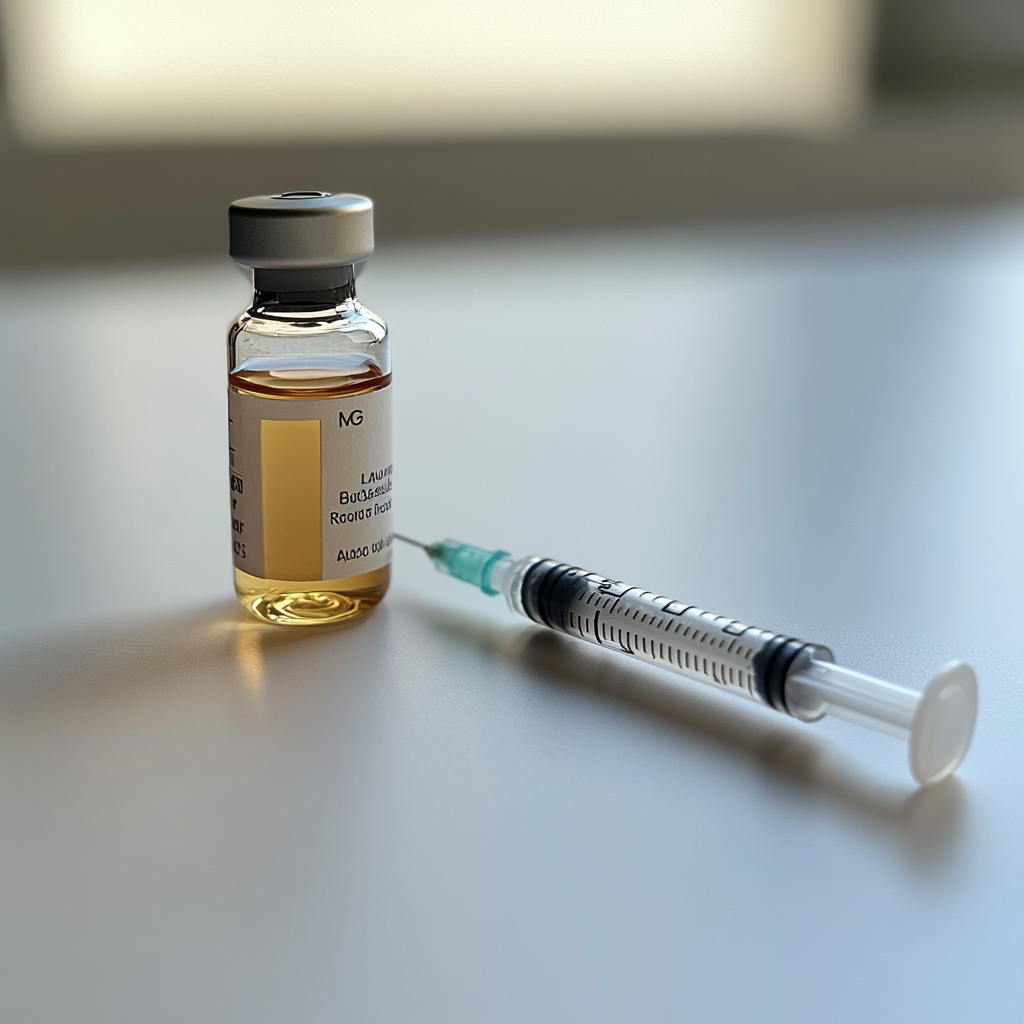
\includegraphics[scale=0.1, valign=m]{imgs/vaccine.png}
		\end{subfigure}
		\qquad\tikz[baseline=-\baselineskip]\draw[ultra thick,->] (-1,0) -- ++ (1,0);\qquad	
		\begin{subfigure}{0.3 \textwidth}
			
\includegraphics[scale=0.1, valign=m]{imgs/infectious.png}
		\end{subfigure}
	\end{figure}

	\vspace{0.5em}
	Epidemiology: Does vaccination reduce the spread of infectious disease?
	}
	\only<3>{
	\begin{figure}
		\begin{subfigure}{0.35 \textwidth}
			
\includegraphics[scale=0.1, valign=m]{imgs/video_game.png}
		\end{subfigure}
		\qquad\tikz[baseline=-\baselineskip]\draw[ultra thick,->] (0,0) -- ++ (1,0);\qquad	
		\begin{subfigure}{0.35 \textwidth}
			
\includegraphics[scale=0.1, valign=m]{imgs/fight.png}
		\end{subfigure}
	\end{figure}
	Social Sciences: Does exposure to violent video games increase aggressive behavior in children?
	}
	\only<4>{
	\begin{figure}
		\begin{subfigure}{0.35 \textwidth}
			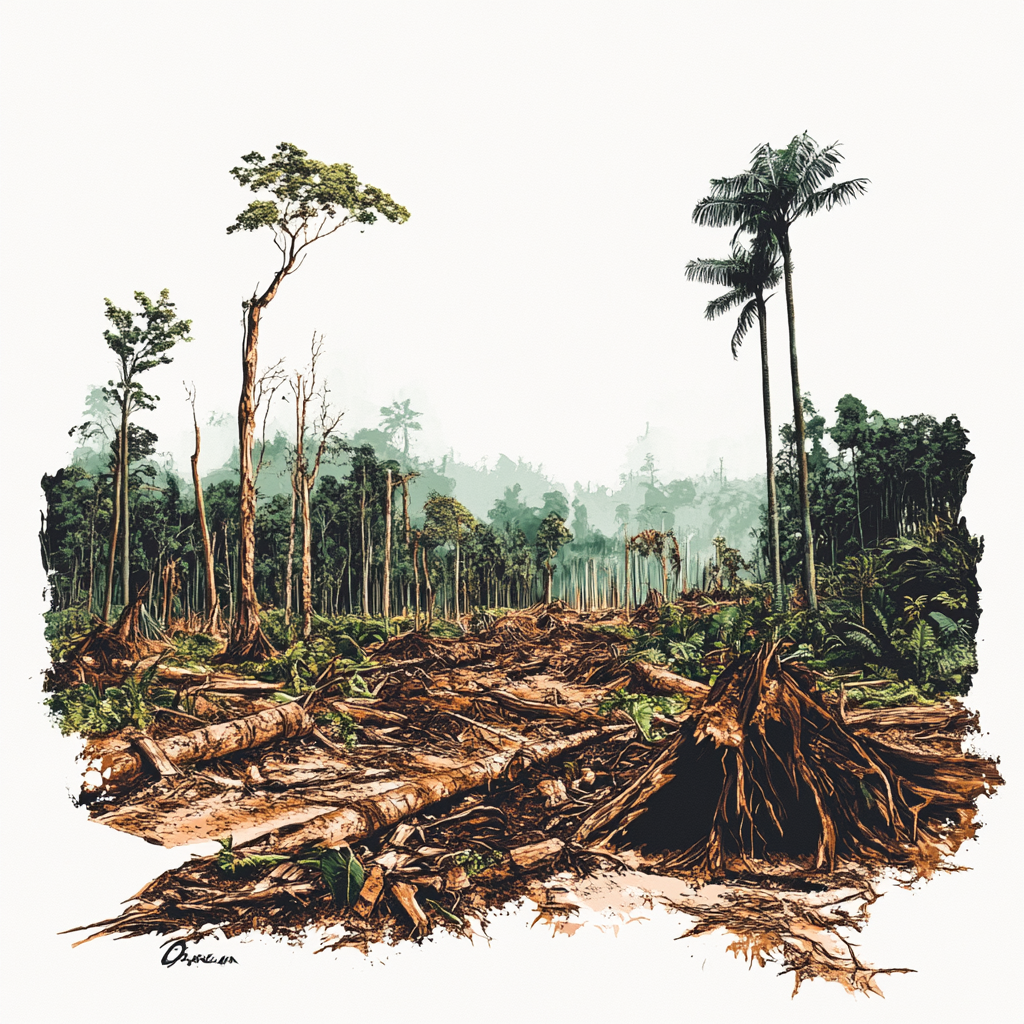
\includegraphics[scale=0.1, valign=m]{imgs/deforestation.png}
		\end{subfigure}
		\qquad\tikz[baseline=-\baselineskip]\draw[ultra thick,->] (0,0) -- ++ (1,0);\qquad	
		\begin{subfigure}{0.35 \textwidth}
			
\includegraphics[scale=0.1, valign=m]{imgs/climate_change.png}
		\end{subfigure}
	\end{figure}

	Environmental Science: Does deforestation contribute to climate change?
	}
\end{frame}

\begin{frame}{Causal Inference}
	\center{Understand how an \textbf{intervention} on an \stackwords{\textbf{exposure}}{vaccination}{video games}{deforestation} influences an \stackwords{\textbf{outcome}.}{infection spread}{aggressive behavior}{climate change}}

	\vspace{2em}

	\begin{itemize}
		\item \textbf{Understanding Causal Relationships: }
			\begin{itemize}
				\item Whether there is a causal relationship between the exposure and the outcome.
				\item Examine the type of relationship such as direct, or indirect.
			\end{itemize}
		\item \textbf{Quantifying Causal Relationships: }
			\begin{itemize}
				\item Measure the magnitude of the intervention's impact.
				\item For example, if we start vaccinating people, by how much would the spread of infection decrease.
			\end{itemize}
	\end{itemize}
\end{frame}

\begin{frame}{Randomized Controlled Trial}	
	\center{Best way to answer these causal questions is using \textbf{Randomized Controlled Trials}.}
	\todo[inline]{Insert a figure here}
\end{frame}

\begin{frame}{Randomized Controlled Trial}
	\center{However, randomized controlled trials are \textbf{not always feasible.}}
	
	\vspace{2em}

	\begin{itemize}[<+->]
		\item \textbf{Unethical: } To study the effect of smoking on lung cancer, we can not ask non-smokers to start smoking.
		\item \textbf{Difficult to control exposures:} To study the effects of deforestation on climate, we can not create a clone of earth.
		\item \textbf{Cost:} Assessing the effect of education on income would require decades of tracking individuals.
	\end{itemize}

	\vspace{2em}

\only<4>{
\center{Can we answer these questions using data that we already have?}}
\end{frame}

\begin{frame}{Causal Graphs}
	\center{Yes, requires understanding the causal mechanism.}
	\vspace{1em}
	% \begin{overprint}
	% 	\onslide<1>\begin{figure} \includegraphics[page=1]{figures.pdf} \end{figure}
	% 	\onslide<2>\begin{figure} \includegraphics[page=2]{figures.pdf} \end{figure}

	% \end{overprint}
	\begin{figure}
		\begin{overprint}
			\onslide<1> \center \includegraphics[page=1]{figures.pdf}
			\onslide<2> \center \includegraphics[page=2]{figures.pdf}
			\onslide<3> \center \includegraphics[page=3]{figures.pdf}
			\onslide<4> \center \includegraphics[page=4]{figures.pdf}
		\end{overprint}
	\end{figure}

	\vspace{1em}
\only<4>{
	\begin{enumerate}
		\item Understanding Causal Relationship $ \implies $ Constructing causal graph.
		\item Quantifying causal relationships $ \implies $ Estimating edge strength.
	\end{enumerate}
}
\end{frame}

% \begin{frame}{Mixed and Missing Data}
% 	\center{I have focused on improving these methods for mixed and missing data.}
% 
% 	\vspace{2em}
% 
% 	\begin{itemize}
% 		\item \textbf{Mixed Data:}
% 			\begin{enumerate}
% 				\item Numerical:
% 				\item Categorical:
% 				\item Ordinal:
% 			\end{enumerate}
% 
% 		\item \textbf{Missing Data:} Not all variables can be measured. For example climate change.
% 	\end{itemize}
% \end{frame}

\begin{frame}{Constructing Causal Graphs}
\center{How to construct causal graphs? Usually done manually.}

\begin{figure}
	\includegraphics[page=1]{figures.pdf}
\end{figure}

\center{Important to test whether our causal graph is correct.}
	
\end{frame}

\begin{frame}{Testing Casual Graphs}
	\todo[inline]{Add a figure showing Independence statements going in to a test and ticks and crosses coming out}

	However, selecting the correct conditional independence test depends on a lot of factors or data needs to be preprocessed.

	We presented a practical guide for researchers trying to apply these methods in their research on how to carry out this testing.
\end{frame}

\begin{frame}{Constructing Causal Graphs}
	\todo[inline]{Insert an image with Data -> Tests -> Causal Graph}

	Model testing relies on these statistical Conditional independence tests.
	Conditional Independence tests can also be used for constructing these graphs
	automatically.

	Hence, important that these tests are accurate.
\end{frame}

\begin{frame}{Causal Effect Estimation}
	If variables can be measured, we have methods to estimate the casual effect between them.

	But some variable can not be directly measured. Example Climate Change.

	These variables are measured indirectly through other variables. For example climate change can be measured through "Global Average Temperature", "Sea Level Rise", "Atmospheric CO2 concentration".

	We developed a new method to be able to estimate these edges.
\end{frame}

\begin{frame}{Software}
	\todo[inline]{If there is time finish this slide}
	To make it easy for these methods to use, we have a software package.
\end{frame}

\begin{frame}{Future research}	
\end{frame}

\begin{frame}
	\Huge{Thank you}
\end{frame}

\end{document}
